\chapter{Обзор средств в области планирования}
    
\section{Средство itSIMPLE}
    Одной из сред поддержки процессов, связанных с планированием, является среда itSIMPLE \cite{itsimple} (Integrated Tools Software Interface for Modeling PLanning Environments).
 В ней предложено использовать UML-модели со специальной семантикой некоторых элементов.
 Описанные модели можно автоматически транслировать на PDDL, а затем подать на вход планировщикам.
 Полученный план затем можно визуализировать внутри среды.
 Под визуализацией понимается отображение в виде диаграмм объектов последовательных состояний, через которые проходит система.
 Так или иначе, средство решает обратную задачу, а не задачу, поставленную в данной работе.
    
    На Рис. \ref{img:its_phil_domain} показано описание классов предметной области  "Обедающие философы".
 С помощью диаграмм состояний в itSIMPLE можно описать, в каких состояниях может находиться объект и как осуществляются переходы между ними.
 Описания переходов не совсем соответствуют спецификации UML, в частности, переходы показаны как методы с параметрами.
 Тем не менее у переходов существуют охранные условия (предусловия) и действия (эффекты), которые задаются на языке OCL.
 На Рис. \ref{img:its_phil_precond} и Рис. \ показаны диаграмма состояний и пример описания предусловий на OCL.

    
    \begin{figure}[h]
        \center{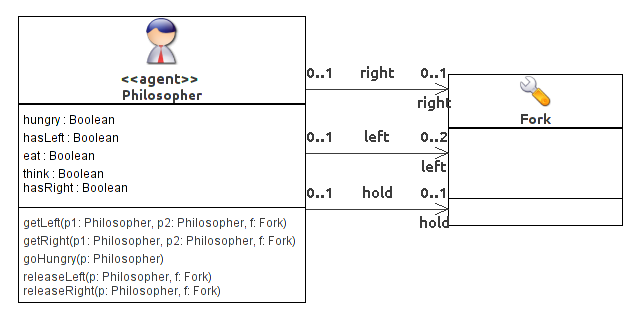
\includegraphics[width=1\linewidth]{its_phil_domain}}
        \caption{Пример описания классов предметной области в itSIMPLE}
        \label{img:its_phil_domain}

    \end{figure}
    
    \begin{figure}[h] 
        \center{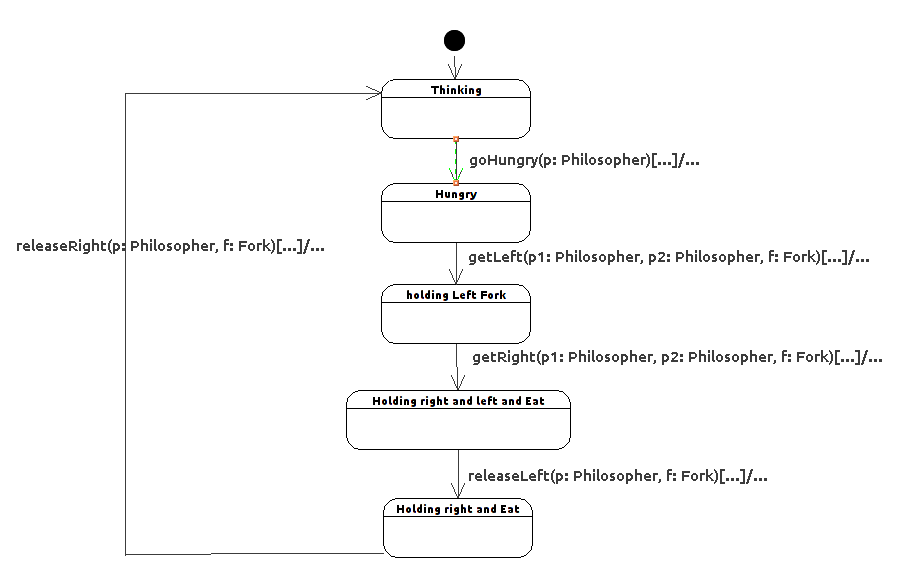
\includegraphics[width=1\linewidth]{its_phil_states}}
        \caption{Пример описания диаграммы состояний объектов в itSIMPLE}
        \label{img:its_phil_states}

    \end{figure}
    
    \begin{figure}[h] 
        \center{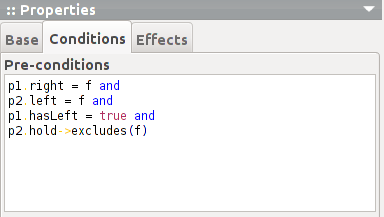
\includegraphics[width=0.5\linewidth]{its_phil_precond}}
        \caption{Пример описания действия \texttt{getRight} в itSIMPLE}
        \label{img:its_phil_precond}

    \end{figure}
        
    
\section{Средство MoDisco}
    Инструмент позволяет создавать модели различных систем, используя специальные Discoverer'ы, которые должны "исследовать" и обработать входные данные.
 На данный момент   Discoverer'ы существуют в основном только для Java-кода и JAR-архивы.
 Кроме того, MoDisco находится в стадии разработки и о скором создании PDDL-Discover'ов говорить не приходится.
 На  Рис. \ref{img:modisco_overview} показан общий вид работы средства.
    
    \begin{figure}[h]
        \center{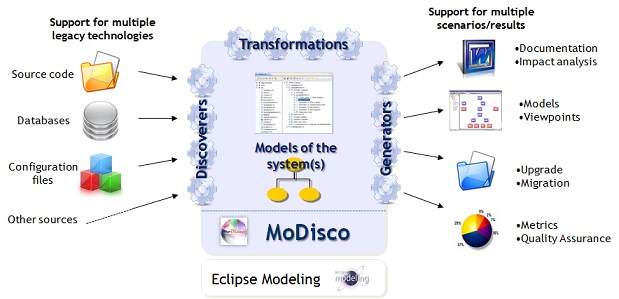
\includegraphics[width=1\linewidth]{modisco_overview}}
        \caption{Схема работы средства MoDisco}
        \label{img:modisco_overview}

    \end{figure}    

\section{Решение задач инженерии знаний средствами объектно-ориентированной  инженерии программного обеспечения}    

В статье \cite{mal-manz} предлагается использовать стандартную нотацию UML и язык объектных ограничений OCL для описания предметных областей и задач планирования.

В рамках статьи было предложено задавать описания предметных областей в виде диаграмм классов UML, а пред- и постусловия~--- в виде ограничений на OCL, начальные условия~--- в виде диаграмм объектов, а цели~--- в виде выражений языка OCL.
 
Также, был предложен способ перевода такой нотации в PDDL-описания для планировщика.
 А сам генератор был реализован на основе программного средства Acceleo, реализующего стандарт MOFM2T\cite{mofm2t}.
 
    
\section{Другие средства}
     Подавляющее большинство инструментов, реализующих преобразование каких-либо текстовых данных в UML-модели, существует для работы с языками программирования, как правило, объектно-ориентированными, а не с языками представления знаний.
 Поэтому, использование этих инструментов для решения поставленной задачи невозможно.
  
    
    В далеком 2005 создавалось средство GIPO (Graphical Interface for Planning with Objects)\cite{gipo}~--- графический интерфейс для планирования с объектами.
 Среди его возможностей было: поддержка классического планирования, HTN (иерархические  сети задач), поддержка длительных действий, различные редакторы для создания описаний предметных областей и задач планирования, статический анализ и динамическое тестирование плана, встроенные и сторонние планировщики и трансляция в PDDL.
 К сожалению, там была предложена своя графическая нотация, не имеющая никакого отношения к UML.
 Ныне проект заброшен.
   
\newpage